\setcounter{section}{7}
\section{Kegelschnitte und Quadriken}

\subsection{Kegelschnitte}

Wie wir im vorherigen Kapitel gesehen haben, können wir die quadratische Form einer symmetrischen Matrix \( A \in \mathbb{R}^{2 \times 2} \) wie folgt schreiben

\begin{equation*}
    q(\mathbf{x}) = \mathbf{x}^T A \mathbf{x}, \quad \mathbf{x} \in \mathbb{R}^2.
\end{equation*}

Für eine solche quadratische Form können wir nun eine Niveaumenge definieren. Eine solche Niveaumenge kann man sich wie einen Schnitt durch unsere quadratische Funktion vorstellen. Mathematisch definieren wir eine solche Niveaumenge mit

\begin{equation*}
    \left\{x \in \mathbb{R}^2: \quad q_A(\mathbf{x}) = 1 \right\}.
\end{equation*}

Die resultierenden Niveaumengen einer quadratischen Funktion, mit zwei Variablen, ergeben dann Kegelschnitte. Abhängig von der Matrix \( A \)  erhalten wir einen der folgenden Kegelschnitte. 

\vspace{\baselineskip}

\begin{figure*}[h]
    \centering
    \begin{tikzpicture}[x=0.75pt,y=0.75pt,yscale=-1,xscale=1]
    
    \draw (329.5,59) node  {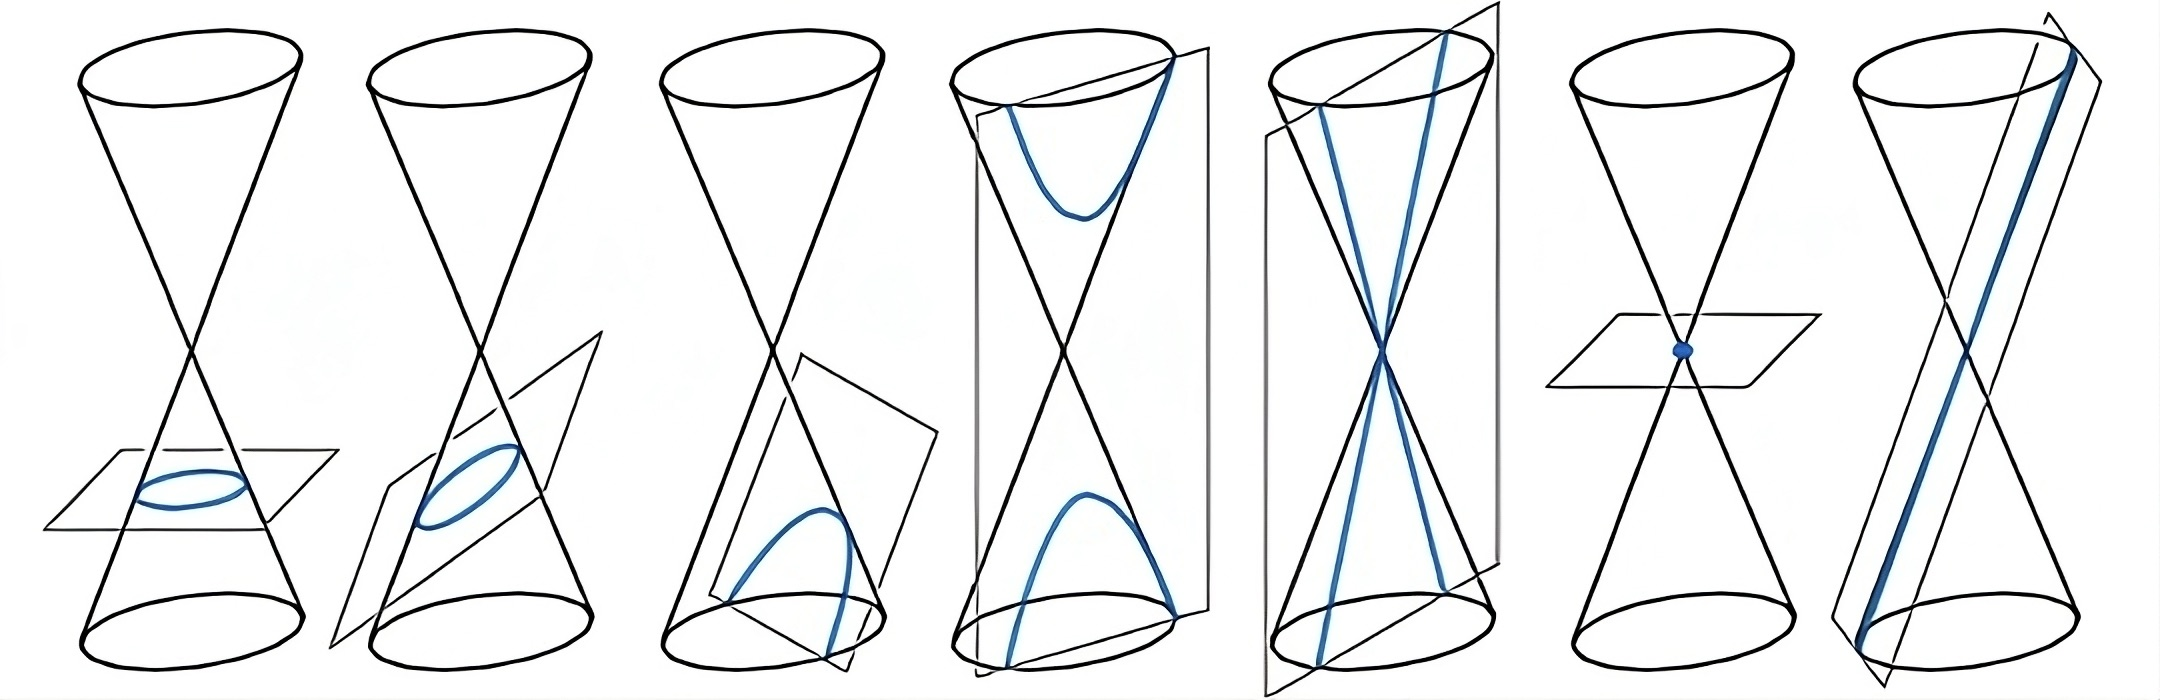
\includegraphics[width=350pt,height=100pt]{media/kegelschnitte.jpeg}};

    \draw (120,130) node [anchor=north west][inner sep=0.75pt]   [align=left] {Kreis};
    \draw (175,130) node [anchor=north west][inner sep=0.75pt]   [align=left] {Ellipse};
    \draw (235,130) node [anchor=north west][inner sep=0.75pt]   [align=left] {Parabel};
    \draw (300,130) node [anchor=north west][inner sep=0.75pt]   [align=left] {Hyperbel};
    \draw (370,130) node [anchor=north west][inner sep=0.75pt]   [align=left] {Geraden};
    \draw (440,130) node [anchor=north west][inner sep=0.75pt]   [align=left] {Punkt};
    \draw (500,130) node [anchor=north west][inner sep=0.75pt]   [align=left] {Gerade};
    \end{tikzpicture}
\end{figure*}

\vspace{\baselineskip}

Zum Beispiel gibt die quadratische Form \( q(\mathbf{x}) = x_1^2 + 4xy + y^2 \), aus der letzten Woche, einen hyperbolischen Kegelschnitt wie wir in der Abbildung sehen können.

\vspace{\baselineskip}

\begin{figure*}[h]
    \centering     
    \begin{tikzpicture}[x=0.75pt,y=0.75pt,yscale=-1,xscale=1]
        %Image [id:dp2813816070099763] 
        \draw (215.5,90.5) node  {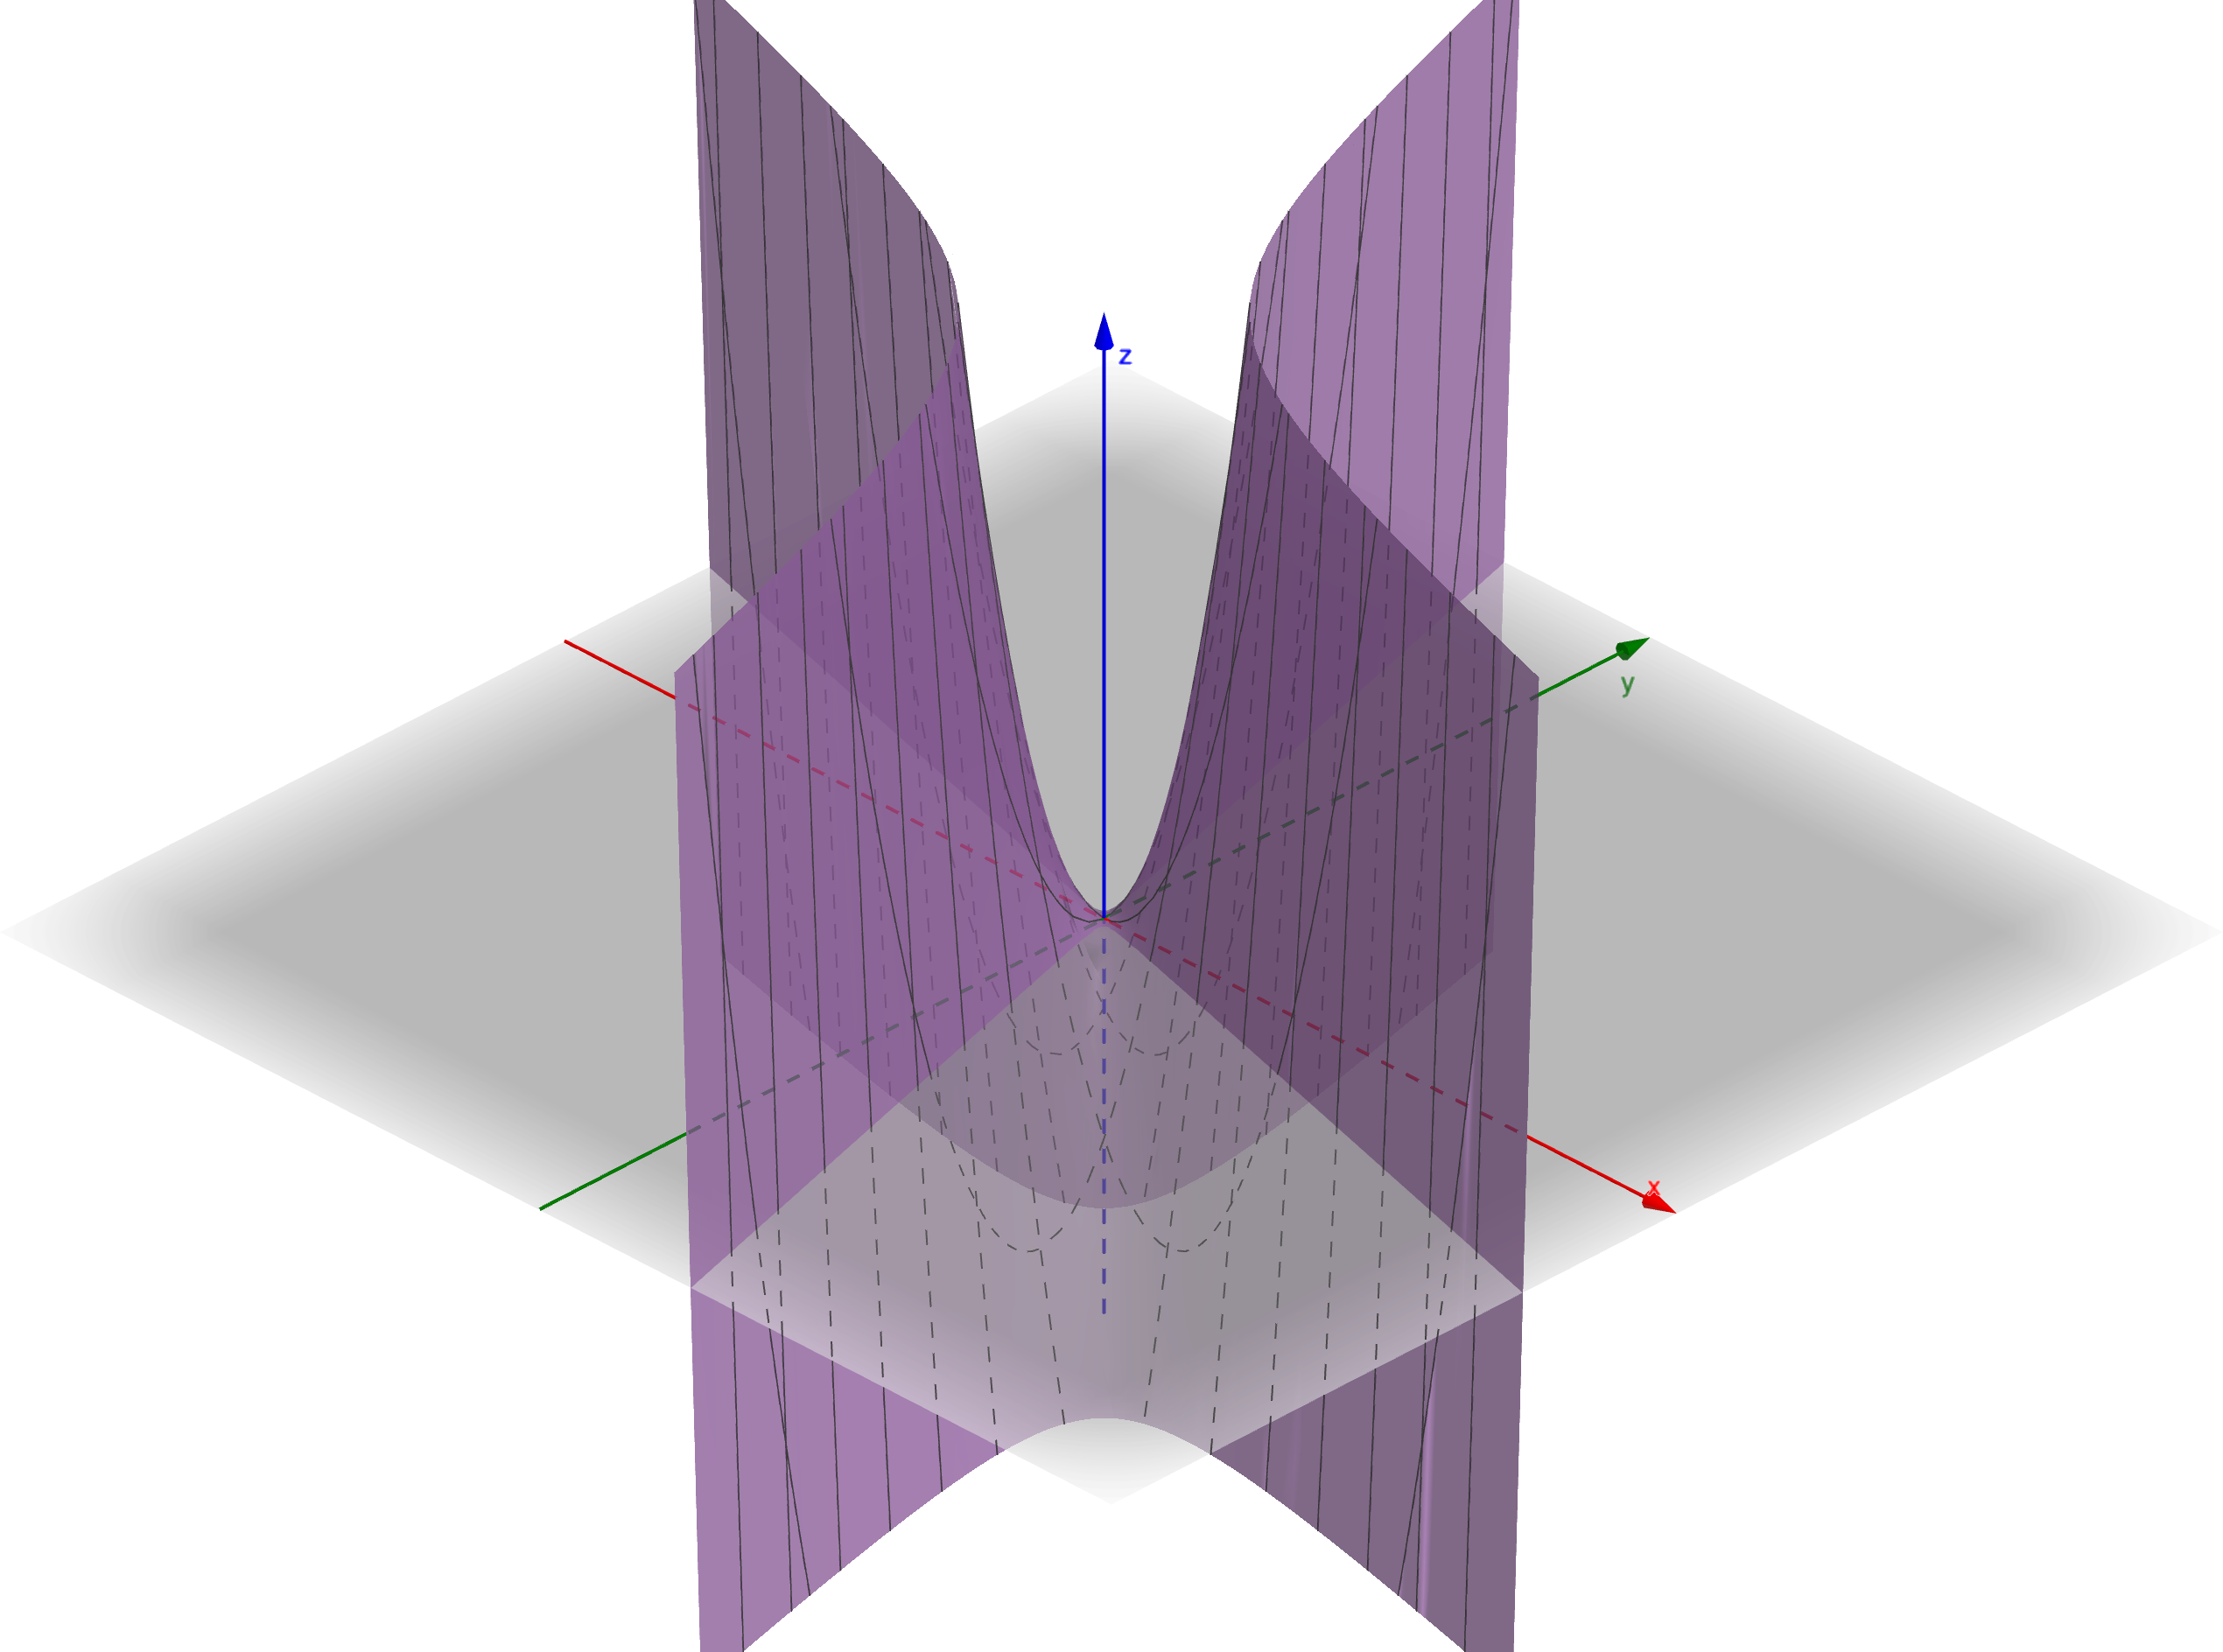
\includegraphics[width=143.25pt,height=120.75pt]{media/kegelschnitt_01.png}};
        %Image [id:dp5757356529933187] 
        \draw (444.75,89.5) node  {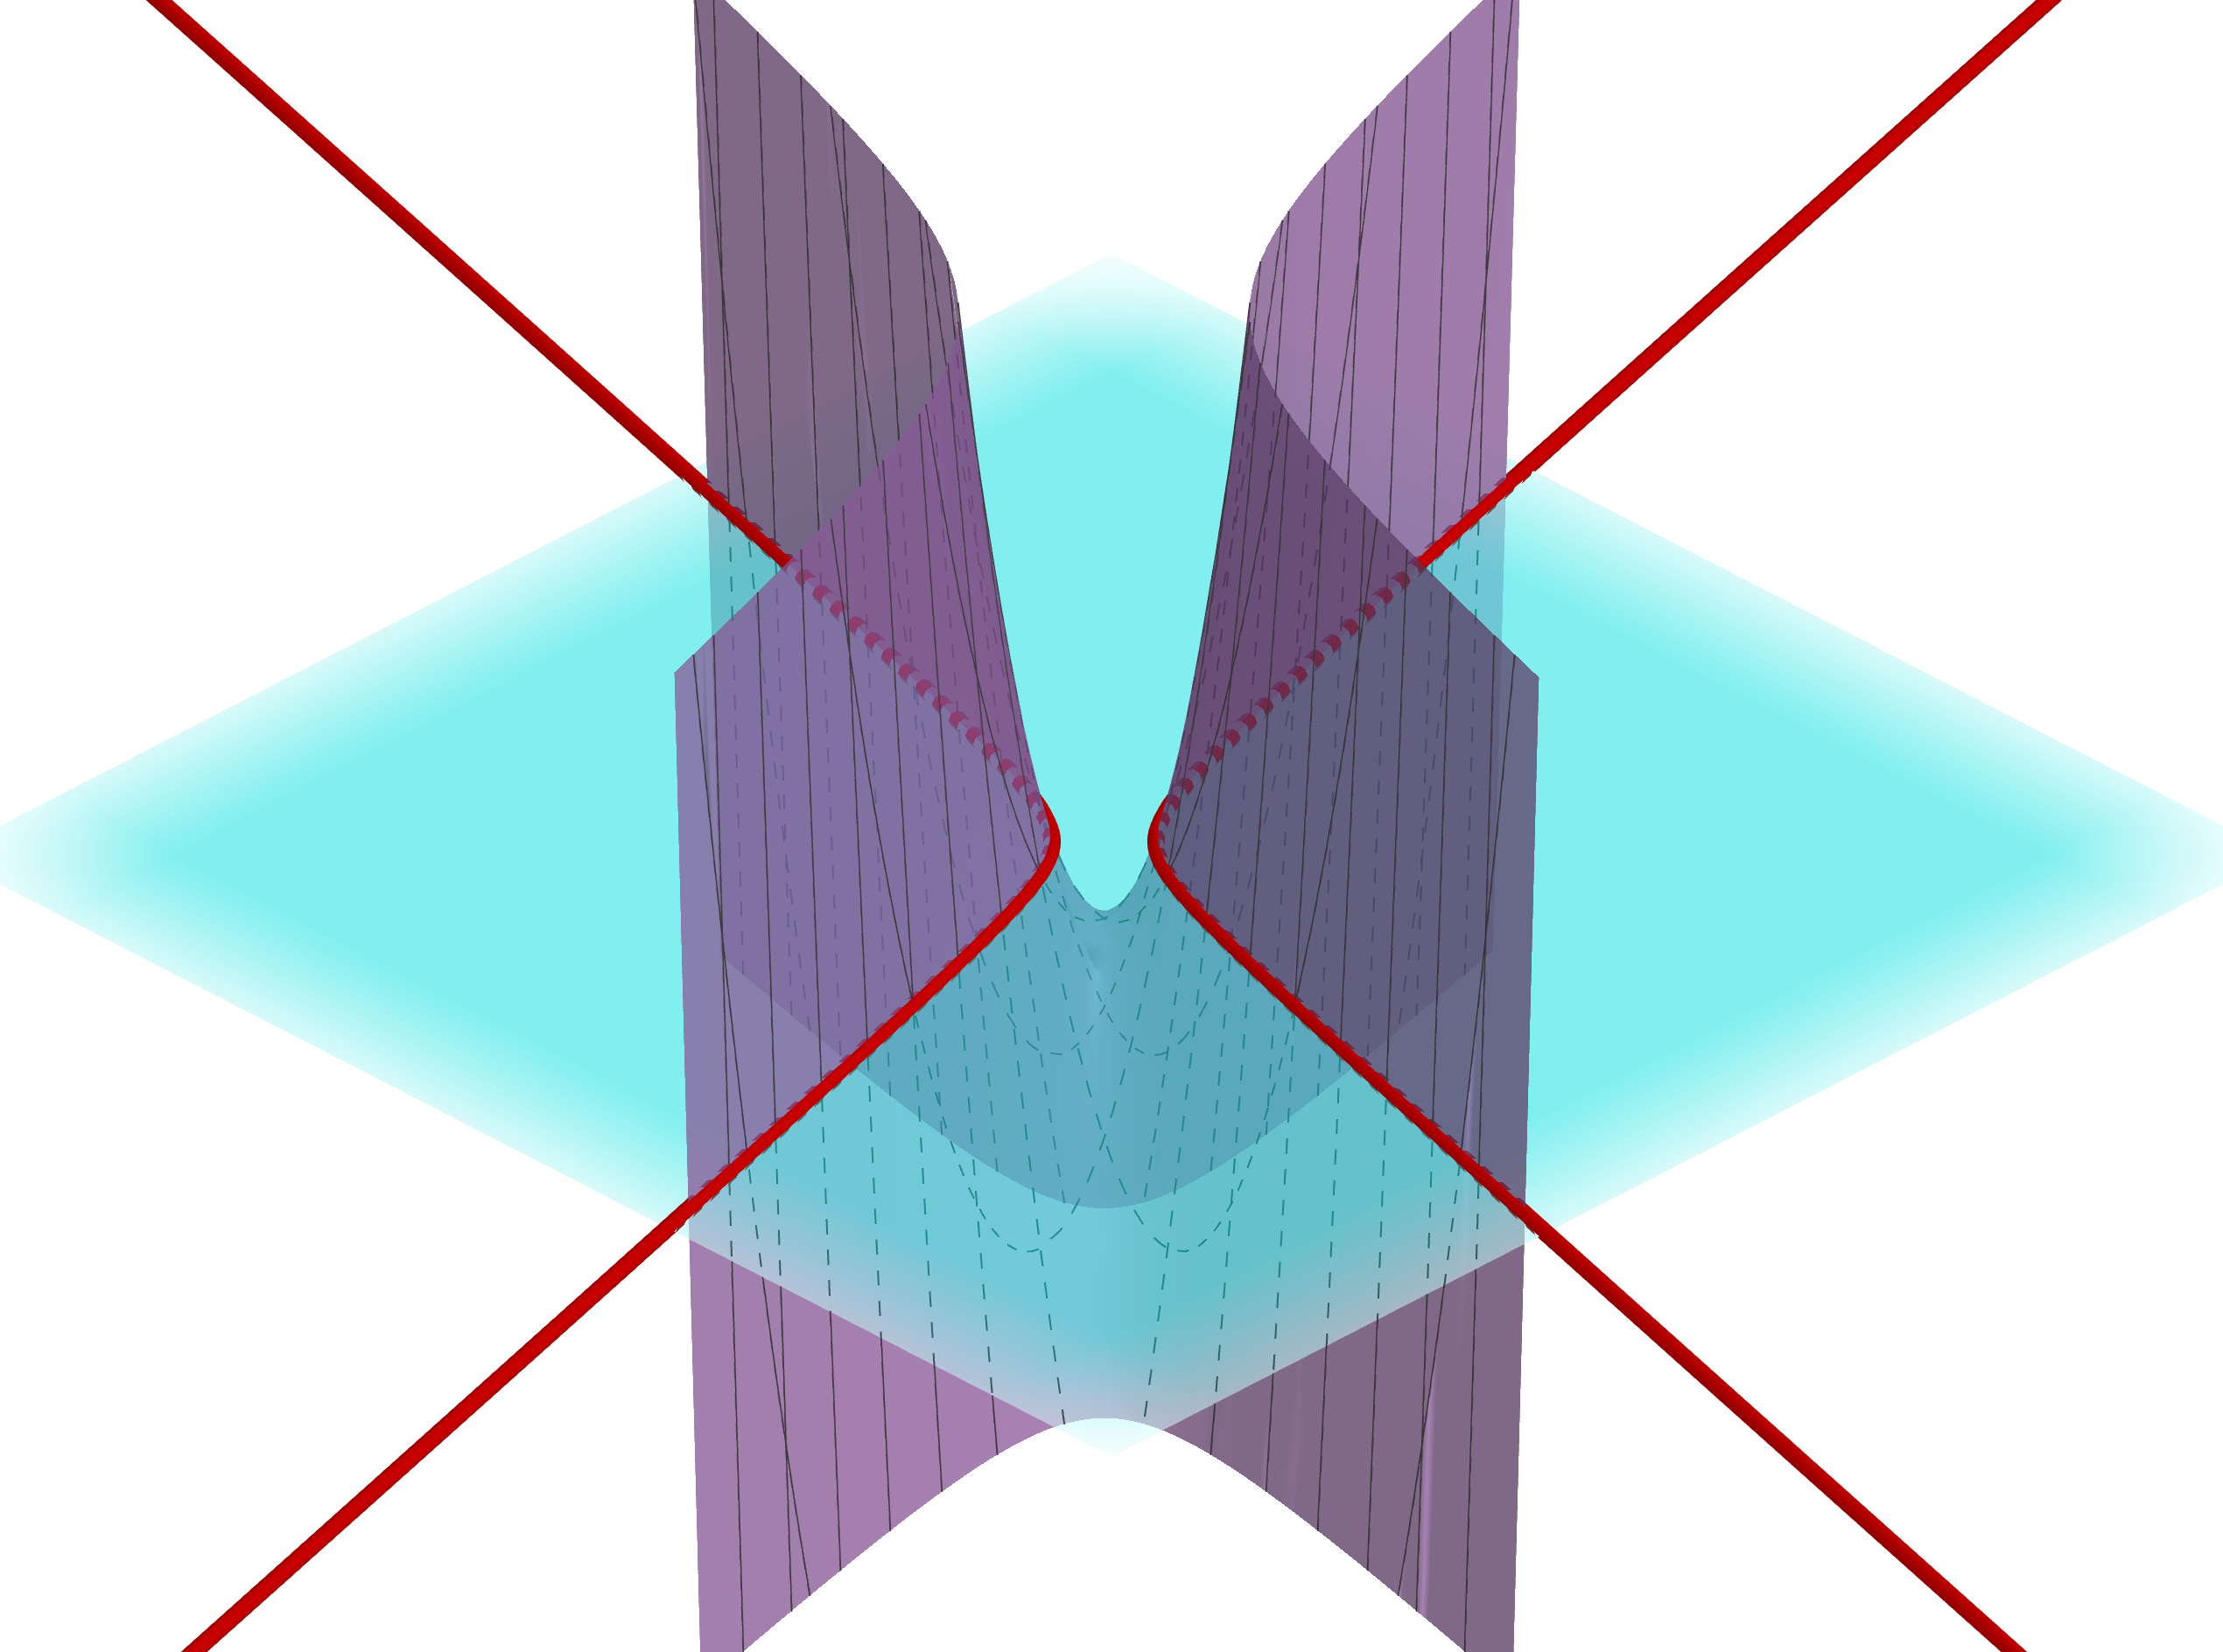
\includegraphics[width=142.13pt,height=120.75pt]{media/kegelschnitt_02.png}};
        %Curve Lines [id:da8140648409741053] 
        \draw    (521.5,53.5) .. controls (514.49,70.33) and (518.4,70.55) .. (507.91,77.46) ;
        \draw [shift={(505.5,79)}, rotate = 327.8] [fill={rgb, 255:red, 0; green, 0; blue, 0 }  ][line width=0.08]  [draw opacity=0] (5.36,-2.57) -- (0,0) -- (5.36,2.57) -- (3.56,0) -- cycle    ;
        %Curve Lines [id:da8764701448468978] 
        \draw    (390,150) .. controls (437.82,150.32) and (439.91,168.38) .. (440,187.05) ;
        \draw [shift={(440,190)}, rotate = 270] [fill={rgb, 255:red, 0; green, 0; blue, 0 }  ][line width=0.08]  [draw opacity=0] (5.36,-2.57) -- (0,0) -- (5.36,2.57) -- (3.56,0) -- cycle    ;
        %Curve Lines [id:da6145373626255732] 
        \draw    (500,150) .. controls (452.82,150) and (450.76,168.35) .. (450.1,187.05) ;
        \draw [shift={(450,190)}, rotate = 271.94] [fill={rgb, 255:red, 0; green, 0; blue, 0 }  ][line width=0.08]  [draw opacity=0] (5.36,-2.57) -- (0,0) -- (5.36,2.57) -- (3.56,0) -- cycle    ;
        % Text Node
        \draw (501.5,36) node [anchor=north west][inner sep=0.75pt]   [align=left] {$\displaystyle z=1$};
        % Text Node
        \draw (406,192) node [anchor=north west][inner sep=0.75pt]   [align=left] {Kegelschnitt};
    \end{tikzpicture}
\end{figure*}

\vspace{\baselineskip}

Ein besonderer Fall ergibt sich, wenn die Matrix \( A \) diagonal ist, dann sind die Hauptachsen des Kegelschnitts parallel zu den Koordinatenachsen. Ein Kegelschnitt im Hauptachsensystem kann in Normalform geschrieben werden. Die Normalformen aller möglichen Kegelschnitte sind in der folgenden Liste gegeben.

\vspace{\baselineskip}

Rang(\( A \)) = 2:

\begin{equation*}
    \begin{aligned}
        & \frac{x^2}{\alpha^2} + \frac{y^2}{\beta^2} - 1 = 0  \quad \text{Ellipse} \\
        & \frac{x^2}{\alpha^2} - \frac{y^2}{\beta^2} - 1 = 0  \quad \text{Hyperbel} \\
        & \frac{x^2}{\alpha^2} + \frac{y^2}{\beta^2} + 1 = 0  \quad \text{leere Menge} \\
        & x^2 + \beta^2 y^2 = 0 \qquad \ \text{Punkt} \\[0.5em]
        & x^2 - \beta^2 y^2 = 0 \qquad \ \text{Geradenpaar} \\
    \end{aligned}
\end{equation*}
        
Rang(\( A \)) = 1:

\begin{equation*}
    \begin{aligned}
        & x^2 - \gamma y = 0 \qquad \text{Parabel} \\
        & x^2 - \alpha^2 = 0 \qquad \text{paralleles Geradenpaar} \\
        & x^2 + \alpha^2 = 0 \qquad \text{leere Menge} \\
        & x^2 = 0 \qquad \qquad \ \text{Gerade} \\
    \end{aligned}
\end{equation*}

\subsection{Quadriken}

Im allgemeinen Fall, wenn \( A \in \mathbb{R}^{n \times n} \) ist, kann die Lösungsmenge der quadratischen Form nicht mehr durch Kegelschnitte beschrieben werden. Im Allgemeinen nennen wir also die Lösungsmenge einer quadratischen Form eine Quadrik. Für den Fall \( n = 3 \) können wir die resultierenden Quadriken noch grafisch als Flächen 2.\ Grades darstellen. Auch hier können wir die Normalformen der Quadriken in einem Hauptachsensystem finden. Einige Beispiele sind:

\vspace{0.5\baselineskip}

\begin{figure*}[h]
    \centering
    \begin{minipage}{0.32\textwidth}
        \centering
        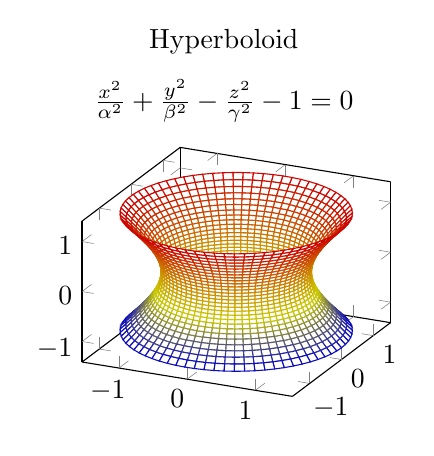
\begin{tikzpicture}
            \begin{axis}[
                width = 5.5cm
            ]
            \addplot3[surf,
                fill=white,
                samples=30,
                samples y=72,
                domain=-1:1,
                y domain=0:360,
                z buffer=sort]
                ( {cosh(x)*cos(y)}, {cosh(x)*sin(y)}, {sinh(x)} );
            \end{axis}
            \draw (1.8,4.5) node [anchor=center][inner sep=0.75pt]   [align=center] {Hyperboloid};
            \draw (1.8,3.75) node [anchor=center][inner sep=0.75pt]   [align=center] {\( \frac{x^2}{\alpha^2} + \frac{y^2}{\beta^2} - \frac{z^2}{\gamma^2} - 1 = 0 \)};
        \end{tikzpicture}
    \end{minipage}
    \hfill
    \begin{minipage}{0.32\textwidth}
        \centering
        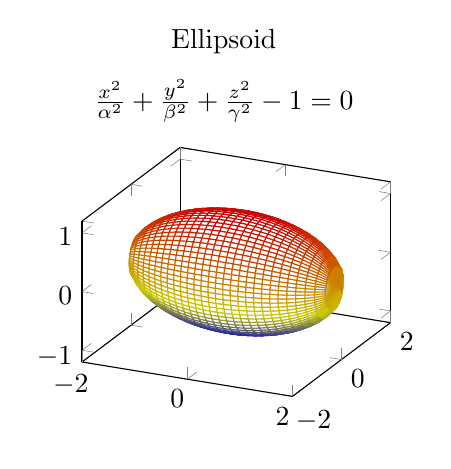
\begin{tikzpicture}
            \begin{axis}[
                width = 5.5cm,
                xmin=-2, xmax=2, 
                ymin=-2, ymax=2,  
            ]
            \addplot3[surf,
                fill=white,
                samples=30,
                samples y=72,
                domain=-1:1,
                y domain=0:360,
                z buffer=sort]
                ({2*x},{cos(y)*sqrt(1-x^2)},{sin(y)*sqrt(1-x^2)});
            \end{axis}
            \draw (1.8,4.5) node [anchor=center][inner sep=0.75pt]   [align=center] {Ellipsoid};
            \draw (1.8,3.75) node [anchor=center][inner sep=0.75pt]   [align=center] {\( \frac{x^2}{\alpha^2} + \frac{y^2}{\beta^2} + \frac{z^2}{\gamma^2} - 1 = 0 \)};
        \end{tikzpicture}
    \end{minipage}
    \hfill
    \begin{minipage}{0.32\textwidth}
        \centering
        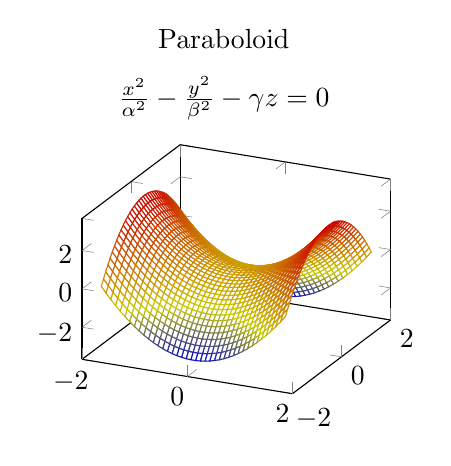
\begin{tikzpicture}
            \begin{axis}[
                width = 5.5cm,
                xmin=-2, xmax=2, 
                ymin=-2, ymax=2
            ]
            \addplot3[surf,
                fill=white,
                samples=40,
                samples y=40,
                domain=-1.75:1.75,
                domain y= -1.75:1.75, 
                z buffer=sort]
                {x^2 - y^2};
            \end{axis}
            \draw (1.8,4.5) node [anchor=center][inner sep=0.75pt]   [align=center] {Paraboloid};
            \draw (1.8,3.75) node [anchor=center][inner sep=0.75pt]   [align=center] {\( \frac{x^2}{\alpha^2} - \frac{y^2}{\beta^2} - \gamma z = 0 \)};
        \end{tikzpicture}
    \end{minipage}
\end{figure*}

Aber wie genau bringen wir quadratische Formen in die entsprechende Normalform?

\subsection{Hauptachsentransformation}

Bei einer Hauptachsentransformation wird ein Kegelschnitt bzw.\ eine Quadrik in die entsprechende Normalform gebracht. Betrachten wir dieses Verfahren an einem Beispiel. 

\vspace{1\baselineskip}

Aufgabe aus der Prüfung Winter 2018. 
\begin{itemize}
    \item Gegeben sei die quadratische Form 

    \begin{equation*}
        q: \mathbb{R}^2 \to \mathbb{R}, \mapsto q(\mathbf{x})=-x_1^2+4x_1x_2-x_2^2.
    \end{equation*}

    Ein Kegelschnitt \( Q \) ist gegeben durch 

    \begin{equation*}
        q(\mathbf{x}) + a^\top \mathbf{x} = 0, \ \text{wobei} \ a^\top = \begin{pmatrix} 6 & -6 \end{pmatrix}.
    \end{equation*}

    Bringen Sie den Kegelschnitt durch eine Hauptachsentransformation \( x = Ty \) und eine Translation auf Normalform, und geben Sie dabei auch \( T \) explizit an. 

\end{itemize}

Betrachten wir zunächst einmal die gegebene quadratische Form \( q(\mathbf{x}) \). Diese lässt sich im 3D Raum darstellen und kann durch eine Matrix \( A \in \mathbb{R}^{2 \times 2} \) beschreiben werden. 

\begin{figure*}[h]
    \centering
    \begin{minipage}{0.32\textwidth}
        \centering
        \begin{equation*}
            A = \begin{pmatrix} -1 & 2 \\ 2 & -1 \end{pmatrix}
        \end{equation*}
        \begin{equation*}
            q(\mathbf{x}) = \mathbf{x}^\top A \  \mathbf{x} 
        \end{equation*}
    \end{minipage}
    \begin{minipage}{0.45\textwidth}
        \centering
        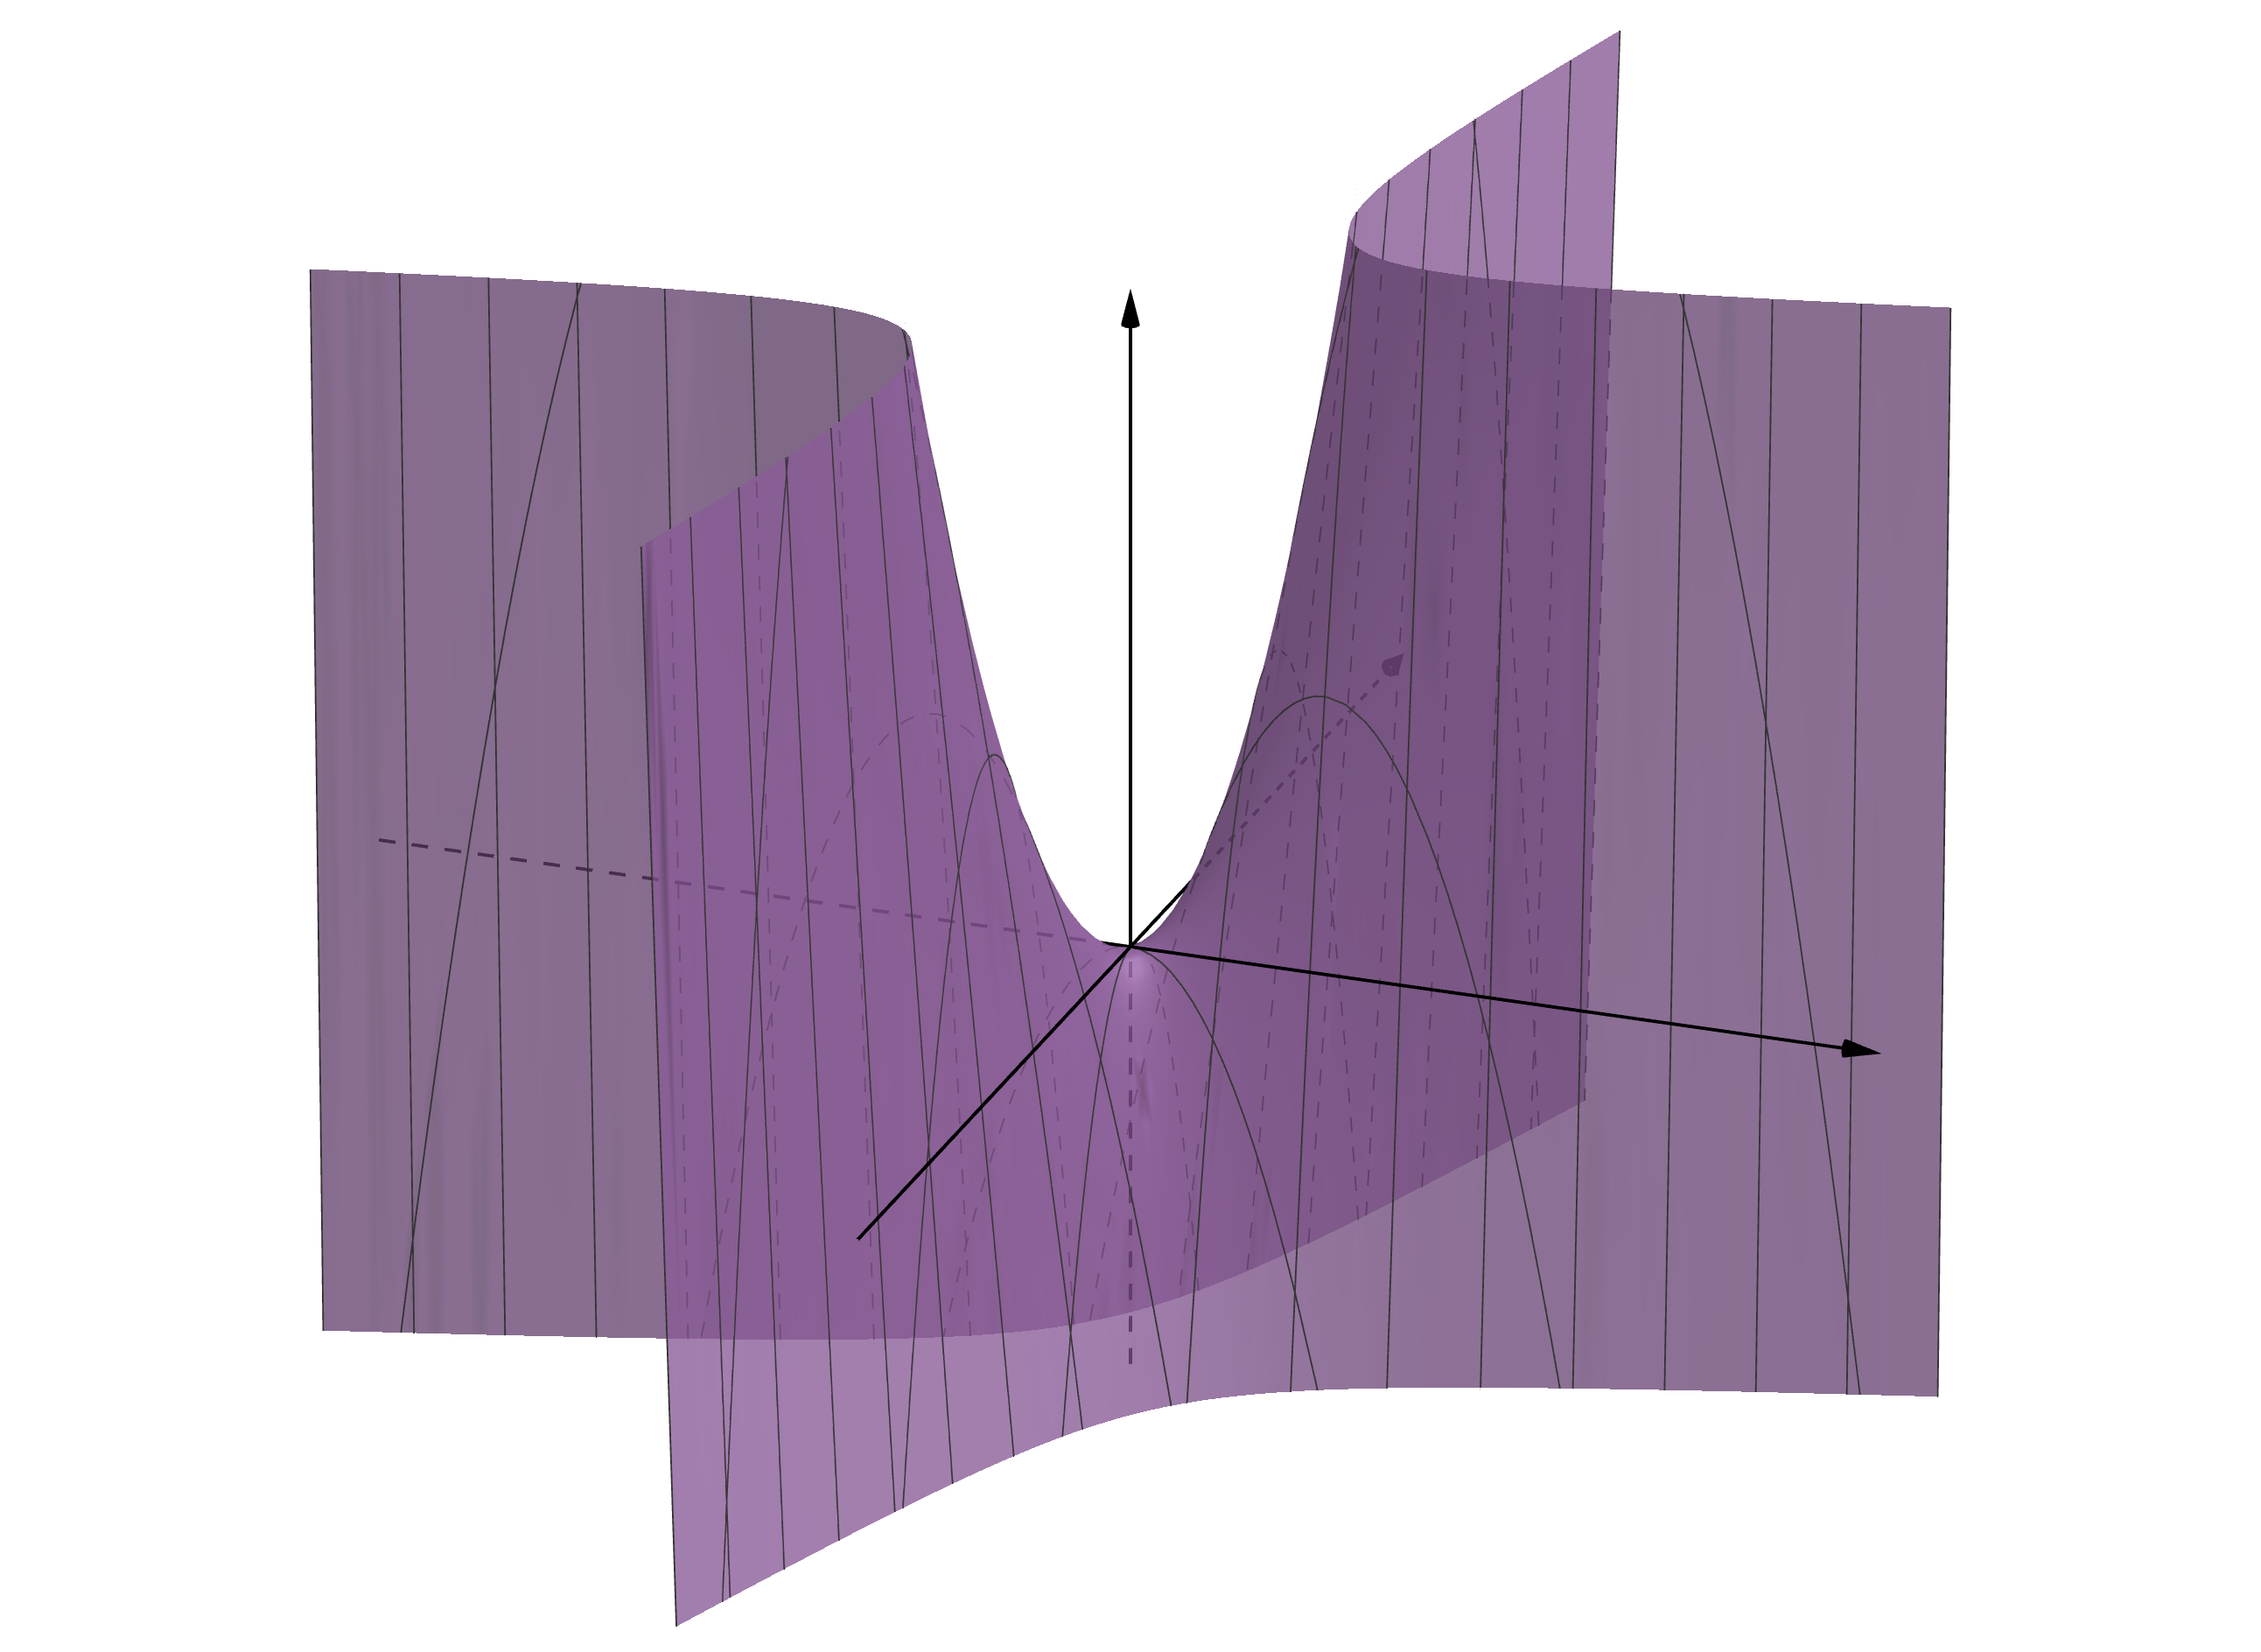
\includegraphics[width=\textwidth]{media/hauptachsen_01.png}
    \end{minipage}
\end{figure*}

Der Kegelschnitt \( Q \) beschreibt die Schnittmenge von \( q(\mathbf{x}) \) mit einer Ebene. In 2 Dimensionen lässt sich die Schnittmenge wie folgt darstellen. 

\begin{figure*}[h]
    \centering
    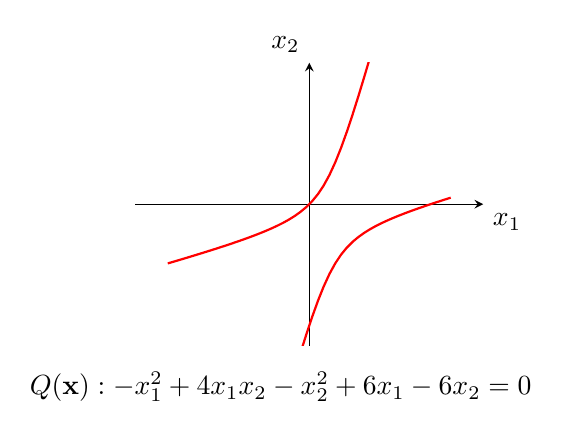
\begin{tikzpicture}[x=0.75pt,y=0.75pt]
        \begin{axis}[
                width = 6cm,
                axis lines = middle,
                xlabel = {\(x_1\)},
                ylabel = {\(x_2\)},
                xlabel style={below right},
                ylabel style={above left}, 
                xmin=-7, xmax=7,
                ymin=-7, ymax=7,
                axis equal,
                xtick=\empty,
                ytick=\empty,
            ]
            \addplot [
                domain=-7:7, 
                samples=50, 
                color=red,
                thick, 
            ]
            {-sqrt(3) * sqrt(x^2 - 2*x + 3) + 2*x - 3};
            \addplot [
                domain=-7:7, 
                samples=50, 
                color=red,
                thick, 
            ]
            {sqrt(3) * sqrt(x^2 - 2*x + 3) + 2*x - 3};
        \end{axis}
        \draw (70,-20) node [anchor=center][inner sep=0.75pt]   [align=center] {\( Q(\mathbf{x}): -x_1^2 + 4x_1x_2 -x_2^2 + 6x_1 - 6x_2 = 0 \)};
    \end{tikzpicture}
\end{figure*}

Zuerst rotieren wir den Kegelschnitt damit die Hauptachsen mit den Koordinatenachsen übereinstimmen. Dazu führen wir einen Basiswechsel \( x = Ty \) durch. In der neuen Basis muss die Matrix \( A \) eine Diagonalmatrix sein. Demnach muss \( A \) diagonalisiert werden. Die dafür benötigten Eigenwerte und Eigenvektoren sind mit 

\begin{equation*}
    \lambda_1 = -3, \quad v_1 = \begin{pmatrix} 1 \\ -1 \end{pmatrix}, \quad \lambda_2 = 1, \quad v_2 = \begin{pmatrix} 1 \\ 1 \end{pmatrix}
\end{equation*}

gegeben. Da wir den Kegelschnitt nur rotieren wollen, ohne seine Form zu verändern, müssen wir unsere Transformationsmatrix \( T \) orthogonal wählen. Dadurch ergibt sich 

\begin{equation*}
    T = \frac{1}{\sqrt{2}} \begin{pmatrix}
        1 & 1 \\
        -1 & 1
    \end{pmatrix}.
\end{equation*}

Nun können wir die Koordinatentransformation durchführen und den Kegelschnitt in der neuen Basis ausdrücken. Per Definition ist \( q(\mathbf{x}) = \mathbf{x}^\top A \mathbf{x} \) wodurch wir \( Q \) umschreiben können.

\begin{equation*}
    Q: q(\mathbf{x}) + a^\top \mathbf{x} = \mathbf{x}^\top A \ \mathbf{x} + a^\top \mathbf{x} = 0
\end{equation*}

Nun setzen wir \( \mathbf{x} = T\mathbf{y} \) ein und erhalten

\begin{equation*}
    \mathbf{x}^\top A \ \mathbf{x} + a^\top \mathbf{x} = \underbrace{(T \mathbf{y})^\top A  \ (T \mathbf{y})}_{\mathbf{y}^\top T^\top A \ T \mathbf{y}} + a^\top T \mathbf{y} = 0
\end{equation*}

Da wir die Matrix \( A \) diagonalisieren und \( T \) orthogonal ist, gilt \( T^\top A T = D \). Der Kegelschnitt vereinfacht sich weiterhin zu 

\begin{equation*}
    \mathbf{y}^\top D \ \mathbf{y} + a^\top T \mathbf{y} = -3y_1^2 + y_2^2 + 6 \sqrt{2} y_1 = 0.
\end{equation*}

Was grafisch, wie erwartet, eine Rotation des Kegelschnitts darstellt.
    
\begin{figure*}[h]
    \centering
    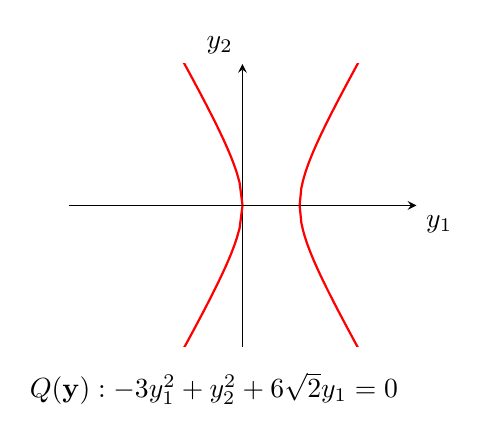
\begin{tikzpicture}[x=0.75pt,y=0.75pt]
        \begin{axis}[
                width = 6cm,
                axis lines = middle,
                xlabel = {\(y_1\)},
                ylabel = {\(y_2\)},
                xlabel style={below right},
                ylabel style={above left}, 
                xmin=-7, xmax=7,
                ymin=-7, ymax=7,
                axis equal,
                xtick=\empty,
                ytick=\empty,
            ]
            \addplot [
                domain=-7:0, 
                samples=50, 
                color=red,
                thick, 
            ]
            { -sqrt(3) * sqrt(x^2 - 2 * sqrt(2) * x)};
            \addplot [
                domain=2.8284:7, 
                samples=50, 
                color=red,
                thick, 
            ]
            { -sqrt(3) * sqrt(x^2 - 2 * sqrt(2) * x)};
            \addplot [
                domain=2.8284:7, 
                samples=50, 
                color=red,
                thick, 
            ]
            { sqrt(3) * sqrt(x^2 - 2 * sqrt(2) * x)};
            \addplot [
                domain=-7:0, 
                samples=50, 
                color=red,
                thick, 
            ]
            { sqrt(3) * sqrt(x^2 - 2 * sqrt(2) * x)};
        \end{axis}
        \draw (70,-20) node [anchor=center][inner sep=0.75pt]   [align=center] {\( Q(\mathbf{y}): -3y_1^2 + y_2^2 + 6 \sqrt{2} y_1 = 0 \)};
    \end{tikzpicture}
\end{figure*}

Um die Normalform zu erhalten, müssen wir nur noch durch eine Translation den \( y_1-\)Term loswerden. Dafür ergänzen wir quadratisch und erhalten

\begin{equation*}
    \begin{aligned}
        0 = & -3y_1^2 + y_2^2 + 6 \sqrt{2} y_1 \\[0.5em]
        = & -3 \left( y_1^2 - 2\sqrt{2} y_1 \right) + y_2^2 \\[0.5em]
        = & -3 \left( \left(y_1 - \sqrt{2}\right)^2 + 2 \right) + y_2^2 \\[0.5em]
        = & -3 \left(y_1 - \sqrt{2}\right)^2 + y_2^2 + 6.
    \end{aligned}
\end{equation*}

Nun wird eine Translation \( \mathbf{z} = \mathbf{y} + \mathbf{c} \) durchgeführt, wobei \( \mathbf{c} \) die Verschiebung in \( y_1 \) Richtung korrigiert. In diesem Fall gilt

\begin{equation*}
    \mathbf{z} = \mathbf{y} + \mathbf{c} = \mathbf{y} + \begin{pmatrix} - \sqrt{2} \\ 0 \end{pmatrix}.
\end{equation*}

Durch einsetzten erhalten wir die Normalform

\begin{equation*}
    \begin{aligned}
        -3z_1^2 + z_2^2 + 6 = 0 \\[0.5em]
        \frac{z_1^2}{2} - \frac{z_2^2}{6} = 1.
    \end{aligned}
\end{equation*}

In der Normalform sehen wir nun eindeutig, dass es sich bei dem Kegelschnitt um eine Hyperbel handelt. Grafisch sieht die Normalform wie folgt aus.

\begin{figure*}[h]
    \centering
    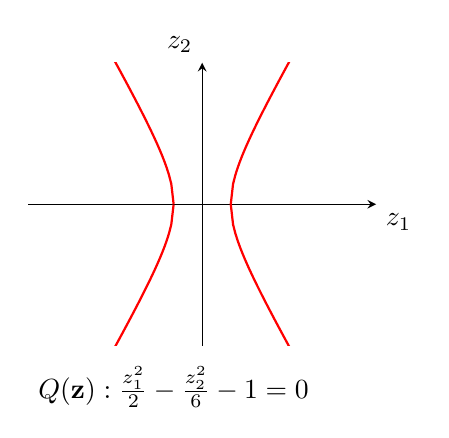
\begin{tikzpicture}[x=0.75pt,y=0.75pt]
        \begin{axis}[
                width = 6cm,
                axis lines = middle,
                xlabel = {\(z_1\)},
                ylabel = {\(z_2\)},
                xlabel style={below right},
                ylabel style={above left}, 
                xmin=-7, xmax=7,
                ymin=-7, ymax=7,
                axis equal,
                xtick=\empty,
                ytick=\empty,
            ]
            \addplot [
                domain=-7:-1.414214, 
                samples=50, 
                color=red,
                thick, 
            ]
            { -sqrt(3) * sqrt(x^2 - 2)};
            \addplot [
                domain=1.414214:7, 
                samples=50, 
                color=red,
                thick, 
            ]
            { -sqrt(3) * sqrt(x^2 - 2)};
            \addplot [
                domain=-7:-1.414214, 
                samples=50, 
                color=red,
                thick, 
            ]
            { sqrt(3) * sqrt(x^2 - 2)};
            \addplot [
                domain=1.414214:7, 
                samples=50, 
                color=red,
                thick, 
            ]
            { sqrt(3) * sqrt(x^2 - 2)};
        \end{axis}
        \draw (70,-20) node [anchor=center][inner sep=0.75pt]   [align=center] {\( Q(\mathbf{z}): \frac{z_1^2}{2} - \frac{z_2^2}{6} - 1  = 0 \)};
    \end{tikzpicture}
\end{figure*}

Wenn wir nun alle Formen vergleichen, ist zu erkennen, dass die Normalform am einfachsten zu interpretieren ist. 

\begin{equation*}
    \begin{aligned}
        Q : & -x_1^2 + 4x_1x_2 - x_2^2 + 6x_1 - 6x_2 = 0 \\[0.5em]
        & -3y_1^2 + y_2^2 + 6\sqrt{2}y_1 = 0 \\[0.5em]
        & \frac{z_1^2}{2} - \frac{z_2^2}{6} - 1 = 0
    \end{aligned}
\end{equation*}